\begin{figure*}[th!]
	\centering
	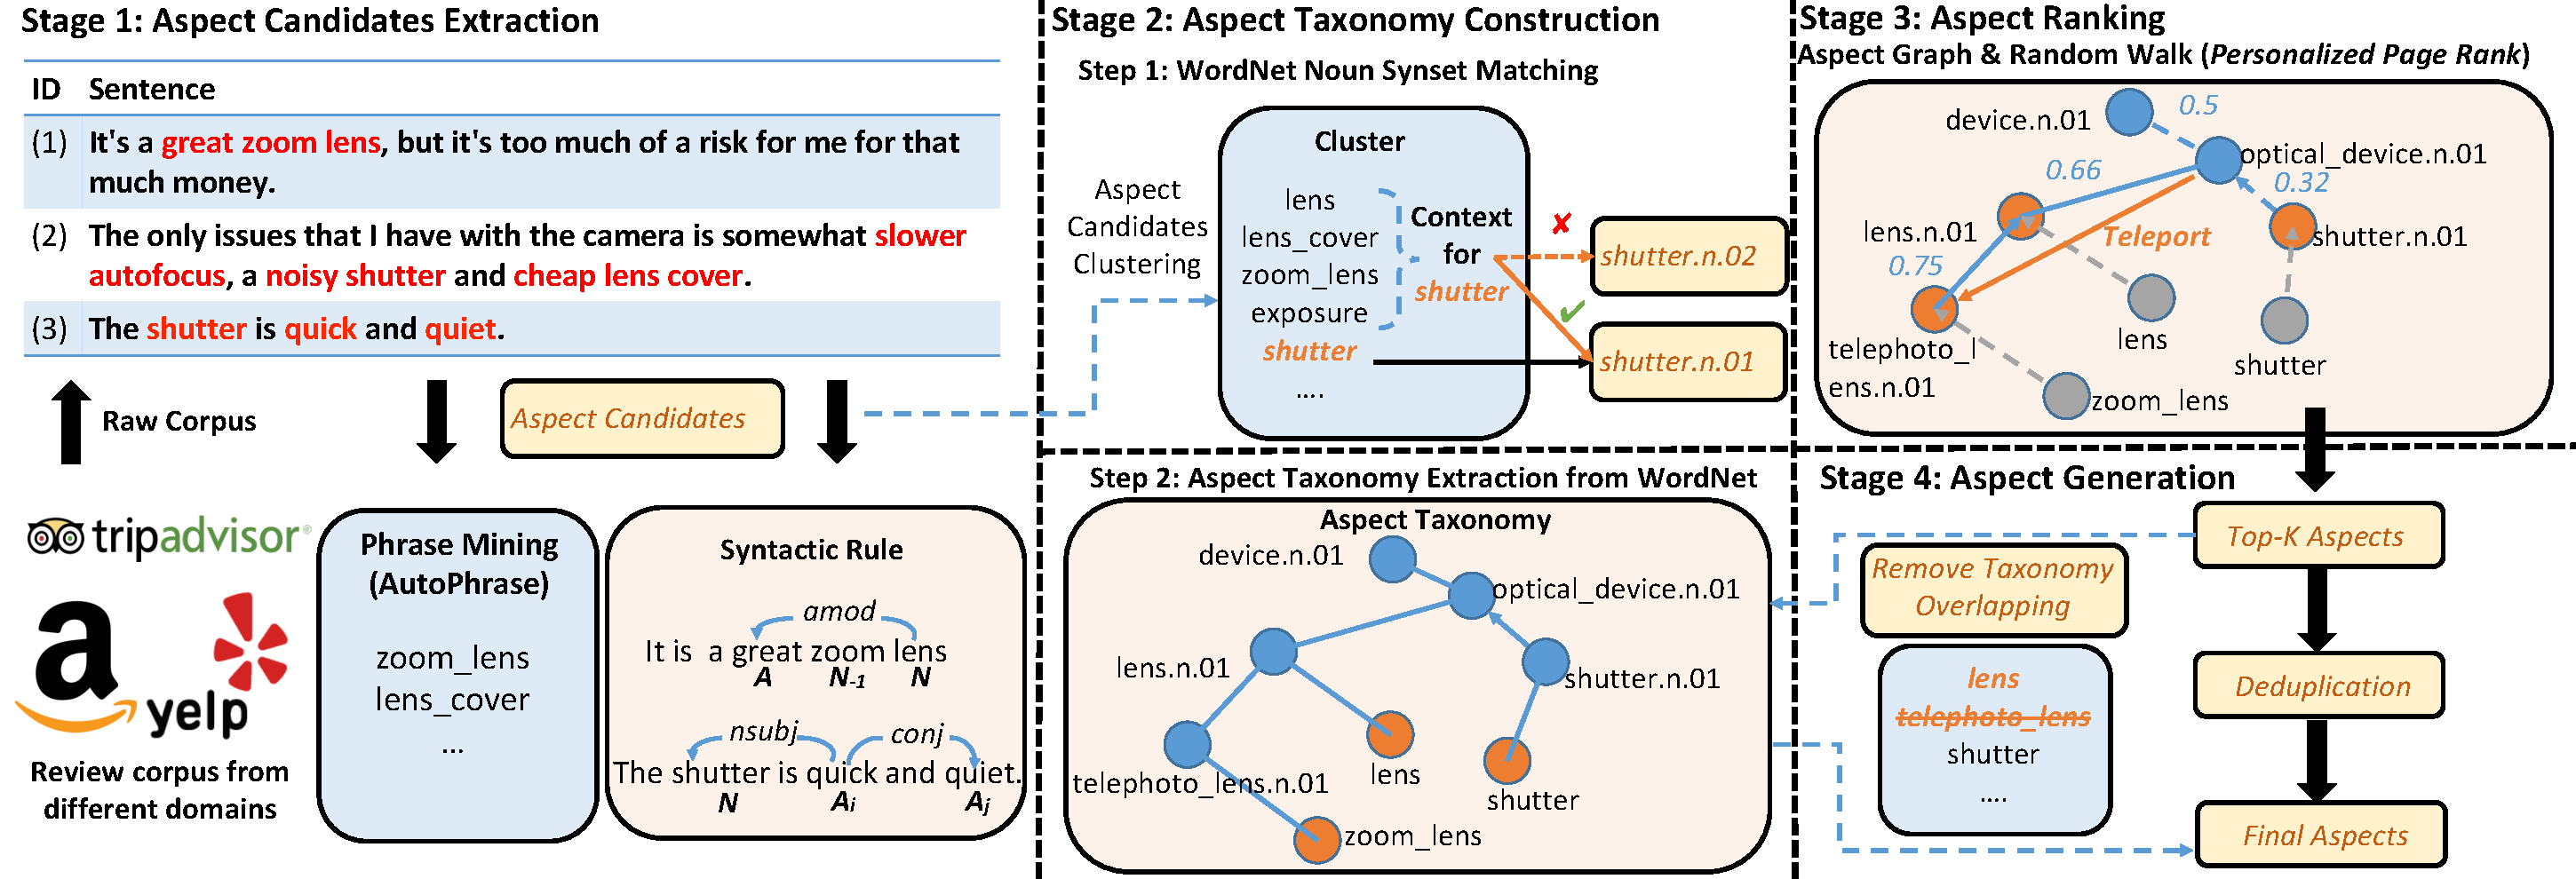
\includegraphics[width=\textwidth]{figures/framework-extra}
	\caption{Overall framework.}
	\label{fig:framework}
\end{figure*}
\section{Framework}
\label{sec:method}
In this section, we first state the \textit{review aspect extraction problem}, 
then present the workflow of our method, shown in \figref{fig:framework}.

\subsection{Problem Statement}
\label{sec:problem}
The review aspect extraction problem is given all the text reviews about
one type of product or service, extract $K$ words (or phrases), 
each of which represents a prominent and distinct review aspect. 

For instance, if the given product type is \textit{hotel}, 
we expect a successful extraction framework to extract 
$K=5$ aspect terms as follows: 
\textit{room, location, staff, breakfast, pool}.
%Here $K$ is an constant parameter for the problem. 
%The set of reviews and the number of aspects are inputs.
%Note that in this definition we don't use cross-domain information, 
%that is, for one product type we only use the reviews of that domain.
%Thus, our model can extract aspects across domains with ease.
%This allows us to apply the model to any domain with ease.

\subsection{Aspect Candidates Extraction}
\label{sec:candidate}
Following the observation of Liu~\shortcite{hu2004mining, liu2015automated}, 
we assume that aspect terms are nouns and noun phrases.  
First, we design a set of effective syntactic rules, which can be applied across domains, to collect the aspect candidates from review texts.
We mainly use the adjectival modifier dependency relation (\emph{amod})
and the nominal subject relation (\emph{nsubj})
to extract the aspect-opinion pairs $\left\langle N, A \right\rangle$.
In addition, we leverage the conjunction relation (\emph{conj}) between 
adjectives to complement the extracted pairs. 
Formally, the extraction rules can be specified as follows:
\begin{description}
	\item[Rule 1.] If $amod(N, A)$, then extract $\left\langle N, A \right\rangle$.
	\item[Rule 2.] If $nsubj(A, N)$, then extract $\left\langle N, A \right\rangle$.
	\item[Rule 3.] If $\left\langle N, A_i \right\rangle$ and $conj(A_i, A_j)$, then extract $\left\langle N, A_j \right\rangle$.
\end{description}
In this case, $N$ indicates a noun, and $A$ (e.g. $A_i$, $A_j$) is an adjective. The dependencies (e.g. $amod(N, A)$) are expressed as \emph{rel(head, dependent)}, where \emph{rel} is the dependency relation which holds between \emph{head} and \emph{dependent}.
Note that many aspects are expressed by phrases, thus,
we extend the phrases as aspect candidates by introducing the extension rules as follows:
\begin{description}
	\item[Rule E1.] If $\left\langle N, A \right\rangle$ and $N_{-1}\_N\in P$, then use $\left\langle N_{-1}\_N, A \right\rangle$ to replace $\left\langle N, A \right\rangle$.
	\item[Rule E2.] If $\left\langle N, A \right\rangle$ and $N\_N_{+1}\in P$, then use $\left\langle N\_N_{+1}, A \right\rangle$ to replace $\left\langle N, A \right\rangle$.
\end{description}
where $N_{-1}$ and $N_{+1}$ denotes the noun word,
and the subscript represents displacement to $N$ in the 
sentence. 
We use AutoPhrase~\cite{liu2017phrase} to extract a set of
phrases $P$ with high coherence.
Then we use $P$ to filter
out the incoherent phrases so as to obtain the high-quality phrases as aspect candidates.
The example in \figref{fig:framework} (Stage 1) demonstrates the extraction process. 
For example, we extract the pair $\langle$ \emph{great}, \emph{zoom\_lens }$\rangle$ from sentence (1) by applying
\emph{Rule 1} and \emph{Rule E1}.
Similarly, the extraction rules match
 $\langle$ \emph{slower}, \emph{autofocus} $\rangle$,
  $\langle$ \emph{noisy}, \emph{shutter} $\rangle$,
   $\langle$ \emph{cheap}, \emph{lens\_cover} $\rangle$ in 
   sentence (2) and 
 $\langle$ \emph{quick}, \emph{shutter} $\rangle$, $\langle$ \emph{quiet}, \emph{shutter} $\rangle$ in sentence (3) as potential aspect-opinion pairs.
After extracting such pairs from the text reviews, 
we sort them by the number of occurrences,
and extract the nouns and noun phrases in the top pairs
as aspect candidates, assuming that
the most prominent aspects are subsumed by those candidates 
terms. 

%\begin{enumerate}
%\item\textit{\ZY{Preprocessing: Derive Synonyms from Wikipedia.}}
%\ZY{We derive those mentions of noun words and mined phrases which have the common transitive target concept as a synonym. Then We substitute the mention to its corresponding synonym in the preprocessing step. }
% 
%\end{enumerate}
%Next we will discuss each stage in more details.


\subsection{Aspect Taxonomy Construction}
\label{sec:taxonomy}
The aspect candidates extracted in the last stage come with the counts 
modified by adjectives. We can directly use such raw counts to rank 
the aspect candidates. This is one of the baseline models in 
our experiments.
However, such ranking usually suffers from the aspect overlapping problem
which obviously violates the principle of pursuing both coverage and 
distinctiveness of prominent aspects.
For example, given the number of prominent aspects 
$K$ as 5,
we can extract both of `location` and `place` aspects from
the hotel reviews. 
In order to solve this problem, we construct an aspect taxonomy 
to obtain such overlapping information between aspect candidates by
leveraging the WordNet ontology. 

\subsubsection{WordNet Synset Matching}
\label{sec:match}
First, we need to match our aspect candidates onto WordNet synsets.
The accuracy of synset matching is very important for our 
aspect taxonomy construction.
This is actually a classical word sense disambiguation (WSD) problem.
Our initial attempt is to use a Python WSD tool~\cite{pywsd14}.
For each aspect candidate, we take it as the target and 
randomly sample a bunch of sentences that contain this target. 
We use the extended word sense disambiguation algorithm~\cite{banerjee2003extended} 
in this tool. We count the total occurrences for each noun 
sense (synset) of the candidate and match the candidate to the most frequent
synset.  However, such a method is not good enough for our problem,
as shown in the results later.
It only considers the local context information within the review sentence. 
Whats more, the review sentences are usually very 
short and colloquial, which makes it 
more difficult to match properly by a common WSD algorithm.
Therefore, it is critical to construct more reliable contexts for 
aspect candidate matching. 

To achieve this goal, we cluster
the aspect candidates with similar semantics together.
Then, for each aspect candidate, 
we take the other candidates within the same cluster
as its context for later disambiguation.
As shown in the first step of stage 2 in \figref{fig:framework}, 
the semantic similar aspect candidates such as 
{\em lens, lens\_cover, zoom\_lens, exposure and shutter}
are clustered together.
For example, we can disambiguate the sense of \emph{shutter} by 
leveraging {\em lens, lens\_cover, zoom\_lens, and exposure}.
We observed that our aspect candidates can be fine-grain 
clustered with a two-stage k-means clustering 
method,\footnote{The implementation details are in \secref{sec:base}.}
which generates the better context for the 
aspect candidates.  More specifically, for a particular aspect candidate $a_t$ 
from the cluster $C = \lbrace a_1, a_2, ..., a_t, ..., a_n \rbrace$, 
we calculate the context vector of $a_t$ as:
\begin{equation}
c(a_t) = \sum_{i=1, i\neq t}^{n} E(a_i),
\end{equation}
where $c(a_t)$ denotes the context vector of $a_t$, 
and $E(a_i)$ represents the embedding of $a_i$.
The set of candidate synsets 
$S(a_t) = \lbrace s^t_1, s^t_2, ..., s^t_m \rbrace$ 
consists of the noun senses (e.g. $s^t_i$) of $a_t$  from WordNet.
Each sense $s^t_i$ is associated with a \emph{gloss} $g^t_i$
(i.e. a brief definition of $s^t_i$) which 
covers the semantics of the sense.
Therefore, we encode $s^t_i$ as the summation
of the word vectors in $g^t_i$:
\begin{equation}
\label{gloss_vec}
v(s^t_i) = \sum_{j=1}^{q} E(w^{t,i}_j),
\end{equation}
$W(g^t_i)$ is the sequence of words in $g^t_i$, i.e., 
$W(g^t_i) = \lbrack w^{t,i}_1, w^{t,i}_2, ..., w^{t,i}_q \rbrack$.
For each candidate sense $s^t_i$ of 
the aspect candidate $a_t$,
we calculate the cosine semantic similarity
between $v(s^t_i)$ and $c(a_t)$, and
match $a_t$ to the most similar $s^t_i$.
%For each synset candidate $s_i$, 
%we calculate its semantic embedding
%by using its gloss definition $G$.
%$G$ is a sequence of words $\lbrace g_1, g_2, ..., g_p\rbrace$

% We compare the accuracies of the above two 
% synset matching methods in our experiments
% to show the effectiveness of our proposed method.

% can be moved to implementation details
%In the first clustering stage, we use the Glove embeddings
%then we leverage the XX embeddings which is learned 
%from the review corpus to capture the \ZY{}
%\ZY{We use the Glove embedding to perform the
%	first-round clustering and the XX embeddings trained on
%	the review texts for the second-round clustering.
%}
%\ZY{Think an ambiguious word to illustrate this}
%\ZY{show some cluster results to illustrate why we need two-stage clustering}
%\ZY{Move this part to implementation details:
% two-stage cluster with different embedding and wiki synonym for 
%embedding training}
%To calculate the similarity between synset gloss and the context of
%aspect candidate, we use the standard pre-trained embeddings (Glove).

\subsubsection{Aspect Taxonomy Extraction from WordNet}
\label{wordnet}
In order to construct the aspect taxonomy from WordNet,
we first extract the hypernym paths for every matched synsets
in the previous step.
By definition, 
a hypernym path $p$ of synset $s$ is the is-a relation path 
from $s$ to the root synset (i.e. entity.n.01 for nouns).
We extract the hypernym paths for each matched synset $s_i$ 
in the WordNet ontology.
Next, we scan over all the collected paths once to construct
the aspect taxonomy which is a directed acyclic graph (DAG).
%More specifically, for each path $p = \lbrack s_1, s_2, ..., s_n \rbrack$,
%we go through the path from $s_1$ to its root synset $s_n$
%and obtain the taxonomy by constructing the is-a relations contained
%in $p$.
In $p$, $s_1$ is the synset matched from our potential aspects,
and $s_{i+1}$ is the hypernym of $s_i$.
As shown in step 2 of Stage 2 in \figref{fig:framework},
we match the aspect candidate \emph{shutter} to \emph{shutter.n.01}.
The only one hypernym path of \emph{shutter.n.01} is 
\emph{[shutter.n.01, optical\_device.n.01, device.n.01, ..., entity.n.01]}.

However, the matched synset usually has multiple hypernym paths 
in WordNet. 
%select those ones which are
%most relevant to the product aspects.
We use the following strategy to compact and minimize the
aspect taxonomy:
\begin{itemize}
	\item Among all the paths from an aspect candidate $s_1$, 
we will keep those paths that contain more than 1 aspect candidates, 
unless there's only one path from $s_1$.
If all paths contain only 1 aspect candidate $s_1$ each, we will keep all of them.

	\item To further optimize the taxonomy structure, we 
induce a minimum subgraph from the original taxonomy using
a heuristic algorithm~\cite{kou1981fast}. Such a subgraph
satisfies the following conditions: 
1) it contains all the nodes matched from aspect candidates;
2) the total number of nodes in the graph is minimal.
Consequently, the induced graph is a weakly connected DAG.
\end{itemize}
%\ZY{We show the effectiveness of 
%	such strategy by sampling the pruned edges which are almost 
%	irrelevant to the aspects. The sampled edges are shown in Table XX. 
%}
After acquiring the aspect taxonomy for the given product or service,
we can now tell if two aspects are semantically overlapped or not. 

\subsection{Aspect Ranking}
\label{sec:rank}
In this section, we propose a novel
method based on personalized page rank 
to compute the overall rank values
for the potential aspects by leveraging the aspect taxonomy.

%\subsubsection{Aspect Graph Formulation}
%\label{sec:graph}
%We adapt the aspect taxonomy to an aspect graph
%on which is able to perform random walk algorithm.
%We reserve the taxonomy structure with directed is-a relations,
%and make the adaption to propagate the aspect importance with 
%intuitive observation.

Let the aspect taxonomy be a graph $G=(V, E)$.
Each node $v\in V$ is a synset in the aspect taxonomy and encoded 
as a vector by instantiating $E$ as Glove embeddings in \eqref{gloss_vec} .
Each edge $e = \langle u, v \rangle$ carries a weight which is
the semantic similarity between the nodes $u$ and $v$,
computed using cosine similarity.
%Note that we can divide the synset vertices $V$ into two categories 
%$V_b$ and $V_w$ ($V=V_b\cup V_w$): 
%\begin{itemize}
%	\item $v\in V_b$ is an aspect candidate synset
%	
%	\item $v \in V_w$ is any other synset.
%\end{itemize}
%We have the following observations:
%\begin{enumerate}
%	\item[\emph{Observation 1}] The synset $v\in V_b$ is matched from the potential aspects,
%	thus the initial aspect importance should propagate from such nodes.
%	\item[\emph{Observation 2}] Besides, such $v\in V_b$ are almost leaves in the graph
%	\footnote{Except for the case that $v_1, v2\in V_b$ and $v_1$ is the hypernym/hypnoym of $v_2$},
%	since we construct the taxonomy using the hypernym paths of 
%	$v\in V_b$.
%	\item[\emph{Observation 3}] The hubs in the aspect graph which have many supporters in $V_b$
%	tend to be more important except for the very general nodes (e.g. abstraction\#n\#06). 
%\end{enumerate}
%According to the first two observations,
%it is reasonable to set the direction of edge $e\in E$ from 
%hypernym to hypnoym in order to facilitate the propagation of
%aspect importance. 
%The third observation inspires us to leverage such structure information 
%for potential aspects ranking. 
%Random walk can achieve this goal.
%In order to prevent the algorithm bias on the very general synsets,
%

%\subsubsection{Random Walks on Aspect Graph}
%\label{sec:random_walk}
Next, we perform the random walks on our constructed
aspect taxonomy.
%According to the first observation in \secref{sec:graph}, 
The propagation starts from candidate aspect nodes in the 
aspect taxonomy, which are called {\em seeds} here.
%We treat such $v\in V_b$ as seeds
%and perform the personalized page rank
%algorithm on the aspect graph 
%to properly boost the aspect importance of the hub nodes
%by leveraging the graph structure.
%
The rank values (aspect importance) of all nodes are:
\begin{equation}
x_t = (1-\alpha)*Ax_{t-1} + \alpha*E \text{,}
\label{eq:ppr}
\end{equation}
%The overall rank is the distribution of the aspect importance
%on each node, which represents by $x_{t-1}$  and $x_{t}$.
where $t$ is the time step in random walk process.
In the initial state $E$(i.e. $x_0$), the aspect importance only distributes on the seeds ($v\in V_b$). 
$E_i$ is the i-th dimension of $E$, indicating
the portion of aspect importance on node $s_i$ 
at time step 0.
$E$ is calculated as follows:
\begin{equation}
E_i = 
\begin{cases}
\frac{f(le(s_i))}{\sum_{j=1}^{n} f(le(s_j))} &  \text{, if $s_i$ is a seed} \\
0 &  \text{, otherwise,}
\end{cases}
\end{equation}
where $n$ is the number of nodes in the graph,
$s_i$ is the synset node,
$le(s_i)$ denotes the lemma form of $s_i$,
and $f(le(s_i))$ represents the frequency that 
$le(s_i)$ is modified by adjectives.

The aspect importance is updated using the transition probabilities matrix 
$A$ which are the normalized weights on the edges of the taxonomy. 
$\alpha$ is the teleport probability, which is 
the probability of returning to the initial distribution
at each time step. 
$\alpha$ determines the distance of propagation of the taxonomy. 
%We empirically to set $\alpha$ as $0.5$ in our experiments.
%which indicates that the expected propagation distance 
%from the seeds is $\frac{1}{\alpha} = 2$.
%We show the effectiveness of this method in  
%quantitative evaluation in \secref{sec:quaneval}.

%\ZY{machine and device}
%\ZY{add the personalized page rank equation here}

\subsection{Aspect Generation}
\label{sec:generation}
Finally, we generate the prominent aspects 
using the rank values of the aspects as well as the is-a relations
in the aspect taxonomy.

We sort $le(s_i)$ in decreasing order by their rank values.
%$le(s_i)$ is the lemma form of synset $s_i$, 
%and $r(s_i)$ is the converged rank values of $s_i$.
We essentially take the top aspects from the sorted list.
However there might be two types of overlapping that we need to
avoid:
i) duplicate: different synset nodes may map to the same aspects, 
i.e., $le(s_i) = le(s_j), s_i \neq s_j$ ( aspects);
ii) taxonomy overlap: the later aspect in the list is the 
hypernym or hyponym of the one of previous aspects.
To this end, we just skip overlapped aspect, and move along the list
until we generate $K$ non-overlapping prominent aspects from the list.

%The end-to-end results in \secref{sec:endeval} show
%the effectiveness of our framework.

%\subsection{Stage 5: Aspect Extraction from Ranked Topic Clusters}
%\label{sec:word_ranking}
%We encode phrases by averaging the embeddings of each words.  
%
%Thus, we encode topic clusters and candidate terms/phrases into a single vector space. 
%It is natural to select the nearest term (word/phrase) to the \textit{AspVec} for each topic cluster base on their cosine similarities.
%The order of extracting follows the ranked list of Stage 3 and 
%we remove each selected term every step, so 
%that the final $K$ prominent aspect terms are unique. 

